%% modified for BE3M33UI at FEL CVUT
%% bare_jrnl.tex
%% V1.2
%% 2002/11/18
%% by Michael Shell
%% mshell@ece.gatech.edu
\documentclass[journal]{IEEEtran}
\usepackage{graphicx}

\begin{document}
%
% paper title
\title{Title ...}
\author{Frank AI}

\markboth{SEMESTRAL WORK, COURSE BE3M33UI, CZECH TECHNICAL UNIVERSITY IN PRAGUE, 20016/17}{Shell \MakeLowercase{\textit{et al.}}: Bare Demo of IEEEtran.cls for Journals}
\maketitle


\begin{abstract}
Short abstract - specify problem, describe your solution and summarize results in a few sentences.
Why shall I read the article?
\end{abstract}

\section{Assignment}
Describe your assignment .

\section{Introduction}
%
Intro to the problem you are solving. A reference to the bibliography item \cite{IEEEhowto:kopka}.

\begin{table}[b]
% increase table row spacing, adjust to taste
\renewcommand{\arraystretch}{1.3}
\caption{An Example of a Table}
\label{table_example}
\centering
% Some packages, such as MDW tools, offer better commands for making tables
% than the plain LaTeX2e tabular which is used here.
\begin{tabular}{|c||c|}
\hline
One & Two\\
\hline
Three & Four\\
\hline
\end{tabular}
\end{table}

\section{Methodology}
Describe algorithms and their configurations, tools used, ...

\section{Experiments}
Describe your experiments here; each figure/table should be explained and interpreted ...
\begin{figure}[!h]
\begin{center}
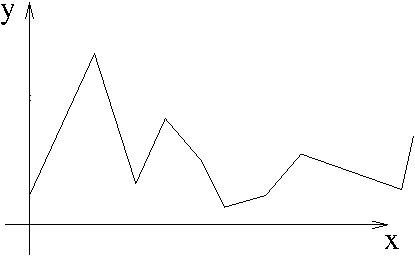
\includegraphics[width=2in]{figure.pdf}
%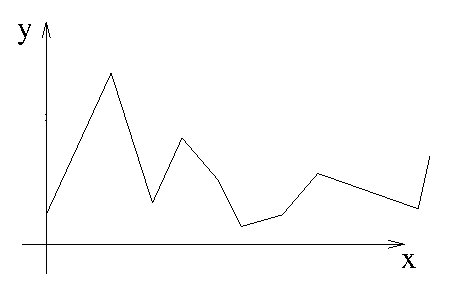
\includegraphics[width=2in]{figure.eps} %to texify use eps
\caption{An example of a graph description.}
\end{center}\label{fig:mypicture}
\end{figure}

\section{Discussion}
Discuss your results here.

\section{Conclusion}
Summary of the work and most important conclusions ...

\begin{thebibliography}{1}

\bibitem{IEEEhowto:kopka}
Author P., Author M.: \emph{Book title}, published by and other info, 2002.

\end{thebibliography}

\end{document}


